
Das entwickelte Framework ist in Unity implementiert und basiert auf einem digitalen
Zwilling des Roboters, der die Zustände der einzelnen Achsen und relevanten
Systemkomponenten kontinuierlich bereitstellt. Darauf aufbauend sind die
Überwachungsmodule (\textit{Monitore}) integriert, die unterschiedliche
Aspekte des Roboterverhaltens beobachten und als Safety Events dokumentieren.


Im Folgenden wird erläutert, wie das Framework funktional, architektonisch und
algorithmisch implemeniert ist. Wichtig dabei sind dabei folgende Annahmen zu
beachten, die sich in Kapitel \ref{sec:aufbauTestszenario} wiederfinden: Als
Testobjekt wird ein ABB IRB 6700-235/2.65 Roboter verwendet. Dabei handelt es
sich um einen Knickarmroboter mit 6 Freiheitsgraden und 6
Gelenken.\vglcite{abbirb2025} Dieser wird in RobotStudio Version 2025.3
simuliert und mittels eines OmniCore-Controllers gesteuert.

\subsection{Funktionale Anforderungen}

Die funktionalen Anforderungen an das Framework
lassen sich in zwei Hauptkategorien unterteilen: die \textbf{Echtzeitüberwachung
	kritischer Roboterzustände} und Programmablaufereignisse sowie die \textbf{systematische
	Protokollierung} der auftretenden Ereignisse.

\subsubsection{Überwachungsfunktionen}

Das Framework muss vier zentrale Überwachungsfunktionen implementieren:

\begin{enumerate}
	\item \textbf{Kollisionserkennung}: Identifikation von Kontakten zwischen Roboterkomponenten und Objekten in der Arbeitsumgebung sowie Selbstkollisionen zwischen benachbarten Gliedern der kinematischen Kette.

	\item \textbf{Singularitätserkennung}: Frühzeitige Erkennung kinematischer Singularitäten (Handgelenk-, Schulter- und Ellbogensingularitäten), die zu Kontrollverlust oder undefinierten Bewegungen führen können.

	\item \textbf{Prozessflussüberwachung}: Validierung der korrekten Abfolge von Bearbeitungsstationen für Werkstücke und Erkennung von Abweichungen von der spezifizierten Sequenz.

	\item \textbf{Gelenkdynamiküberwachung}: Kontinuierliche Überprüfung von Gelenkwinkeln, -geschwindigkeiten und -beschleunigungen auf Grenzwertüberschreitungen, insbesondere während der Handhabung von Werkstücken.
\end{enumerate}

\subsubsection{Systematische Ereignisprotokollierung}

Mithilfe des Frameworks soll es möglich sein, die genannten Fehlerarten
systematisch debuggen zu können und die Fehlersuche in Roboterprogrammcode zu
vereinfachen. Neben der reinen Erkennung ist die folglich eine formalisierte
Dokumentation der Ereignisse notwendig. Jedes detektierte Ereignis soll mit
entsprechenden Metadaten zum aktuellen Status des Roboters angereicht werden.
Folgende Metadaten lassen sich nach initialem Testen mithilfe der zur Verfügung
stehenden Tools extrahieren:

\begin{itemize}
	\item \textbf{Zeitlicher Kontext}: Präziser Zeitstempel des Ereignisses mit Millisekunden-Auflösung
	\item \textbf{Räumlicher Kontext}: Vollständige Gelenkwinkelkonfiguration und TCP-Position zum Ereigniszeitpunkt
	\item \textbf{Programmkontext}: Aktuelles Modul, Routine und Programmzeile der Robotersteuerung
	\item \textbf{Ereignisspezifische Daten}: Je nach Ereignistyp relevante Zusatzinformationen (Kollisionspunkt, Singularitätstyp, Sequenzabweichung, Grenzwertüberschreitung)
\end{itemize}

Diese strukturierte Erfassung ermöglicht die nachgelagerte genaue Auswertung der
vorhandenen Daten und soll das Debuggen des Programmcodes und das Erkennen von
Fehlern im Programmablauf erleichtern.

\subsection{Zielsetzung und architektonische Anforderungen}
Der Stand der Technik aktueller Simulationsplattformen für Roboter zeigt, dass
virtuelle Steuerungen und damit zusammenhängende Simulationsplattformen
herstellerspezifisch entwickelt und mit Ausnahme von ROS keine einheitliche
Schnittstelle zur Kommunikation mit externen Plattformen oder Physik-Engines
bieten. Somit muss für jeden Robotertyp ein designierter Konnektor genutzt
werden, um diesen mit einer externen, herstellerunabhängigen Simulationplattform
zu verbinden. Um eine herstellerunabhängige und erweiterbare Plattform zu
entwickeln, sollte also eine gemeinsame Schnittstelle implementiert werden.


Zusammenfassend verfolgt die Architektur des Frameworks drei zentrale Ziele:
\begin{enumerate}
	\item \textbf{Vendor-Agnostik}: Abstraktion verschiedener Roboterhersteller durch einheitliche Interface-basierte Architektur ohne herstellerspezifische Abhängigkeiten im Kern-Framework

	\item \textbf{Modulare Erweiterbarkeit}: Plugin-System für Safety Monitoring Module und Kommunikationsprotokolle ohne Änderungen der bestehenden Architektur

	\item \textbf{Echtzeitfähige Kommunikation}: Latenzarme Datenübertragung für Motion Control und ereignisbasierte Sicherheitsüberwachung
\end{enumerate}

\subsection{Unity3D als Simulationsplattform}


Unity3D wird in dieser Arbeit ausschließlich als \emph{Simulations\-laufzeit} verwendet.
Die Engine stellt Szene, Physik und Rendering bereit und bietet dank ihrer ausgereiften
3D/Physik‑Infrastruktur eine plattformübergreifende Grundlage für den
digitalen Zwilling des Roboters.\vglcite[247]{andaluz2016} Die eigentliche
Anwendungslogik wird durch klar definierte Adapter von der Engine entkoppelt,
wodurch eine strikte Trennung zwischen Simulation und Domäne gewahrt bleibt.
Asynchrone Abläufe im Update‑Loop dienen lediglich der Taktung und greifen
nicht direkt auf Unity‑APIs zu. Die Wahl von Unity begründet sich zudem durch
die breite Tooling‑Unterstützung und die Möglichkeit, sowohl visuelle als auch
programmatische Arbeitsabläufe zu kombinieren.\vglcite[431]{bartneck2015}


\subsection{Systemarchitektur}

Das entwickelte Framework implementiert eine vierschichtige Architektur, die
eine klare Trennung der Verantwortlichkeiten gewährleistet (siehe Abbildung
\ref{fig:layer_architecture}). Diese Strukturierung folgt etablierten
Software-Engineering-Prinzipien, um Wartbarkeit und Erweiterbarkeit zu
gewährleisten.

\begin{figure}[H]
	\centering
	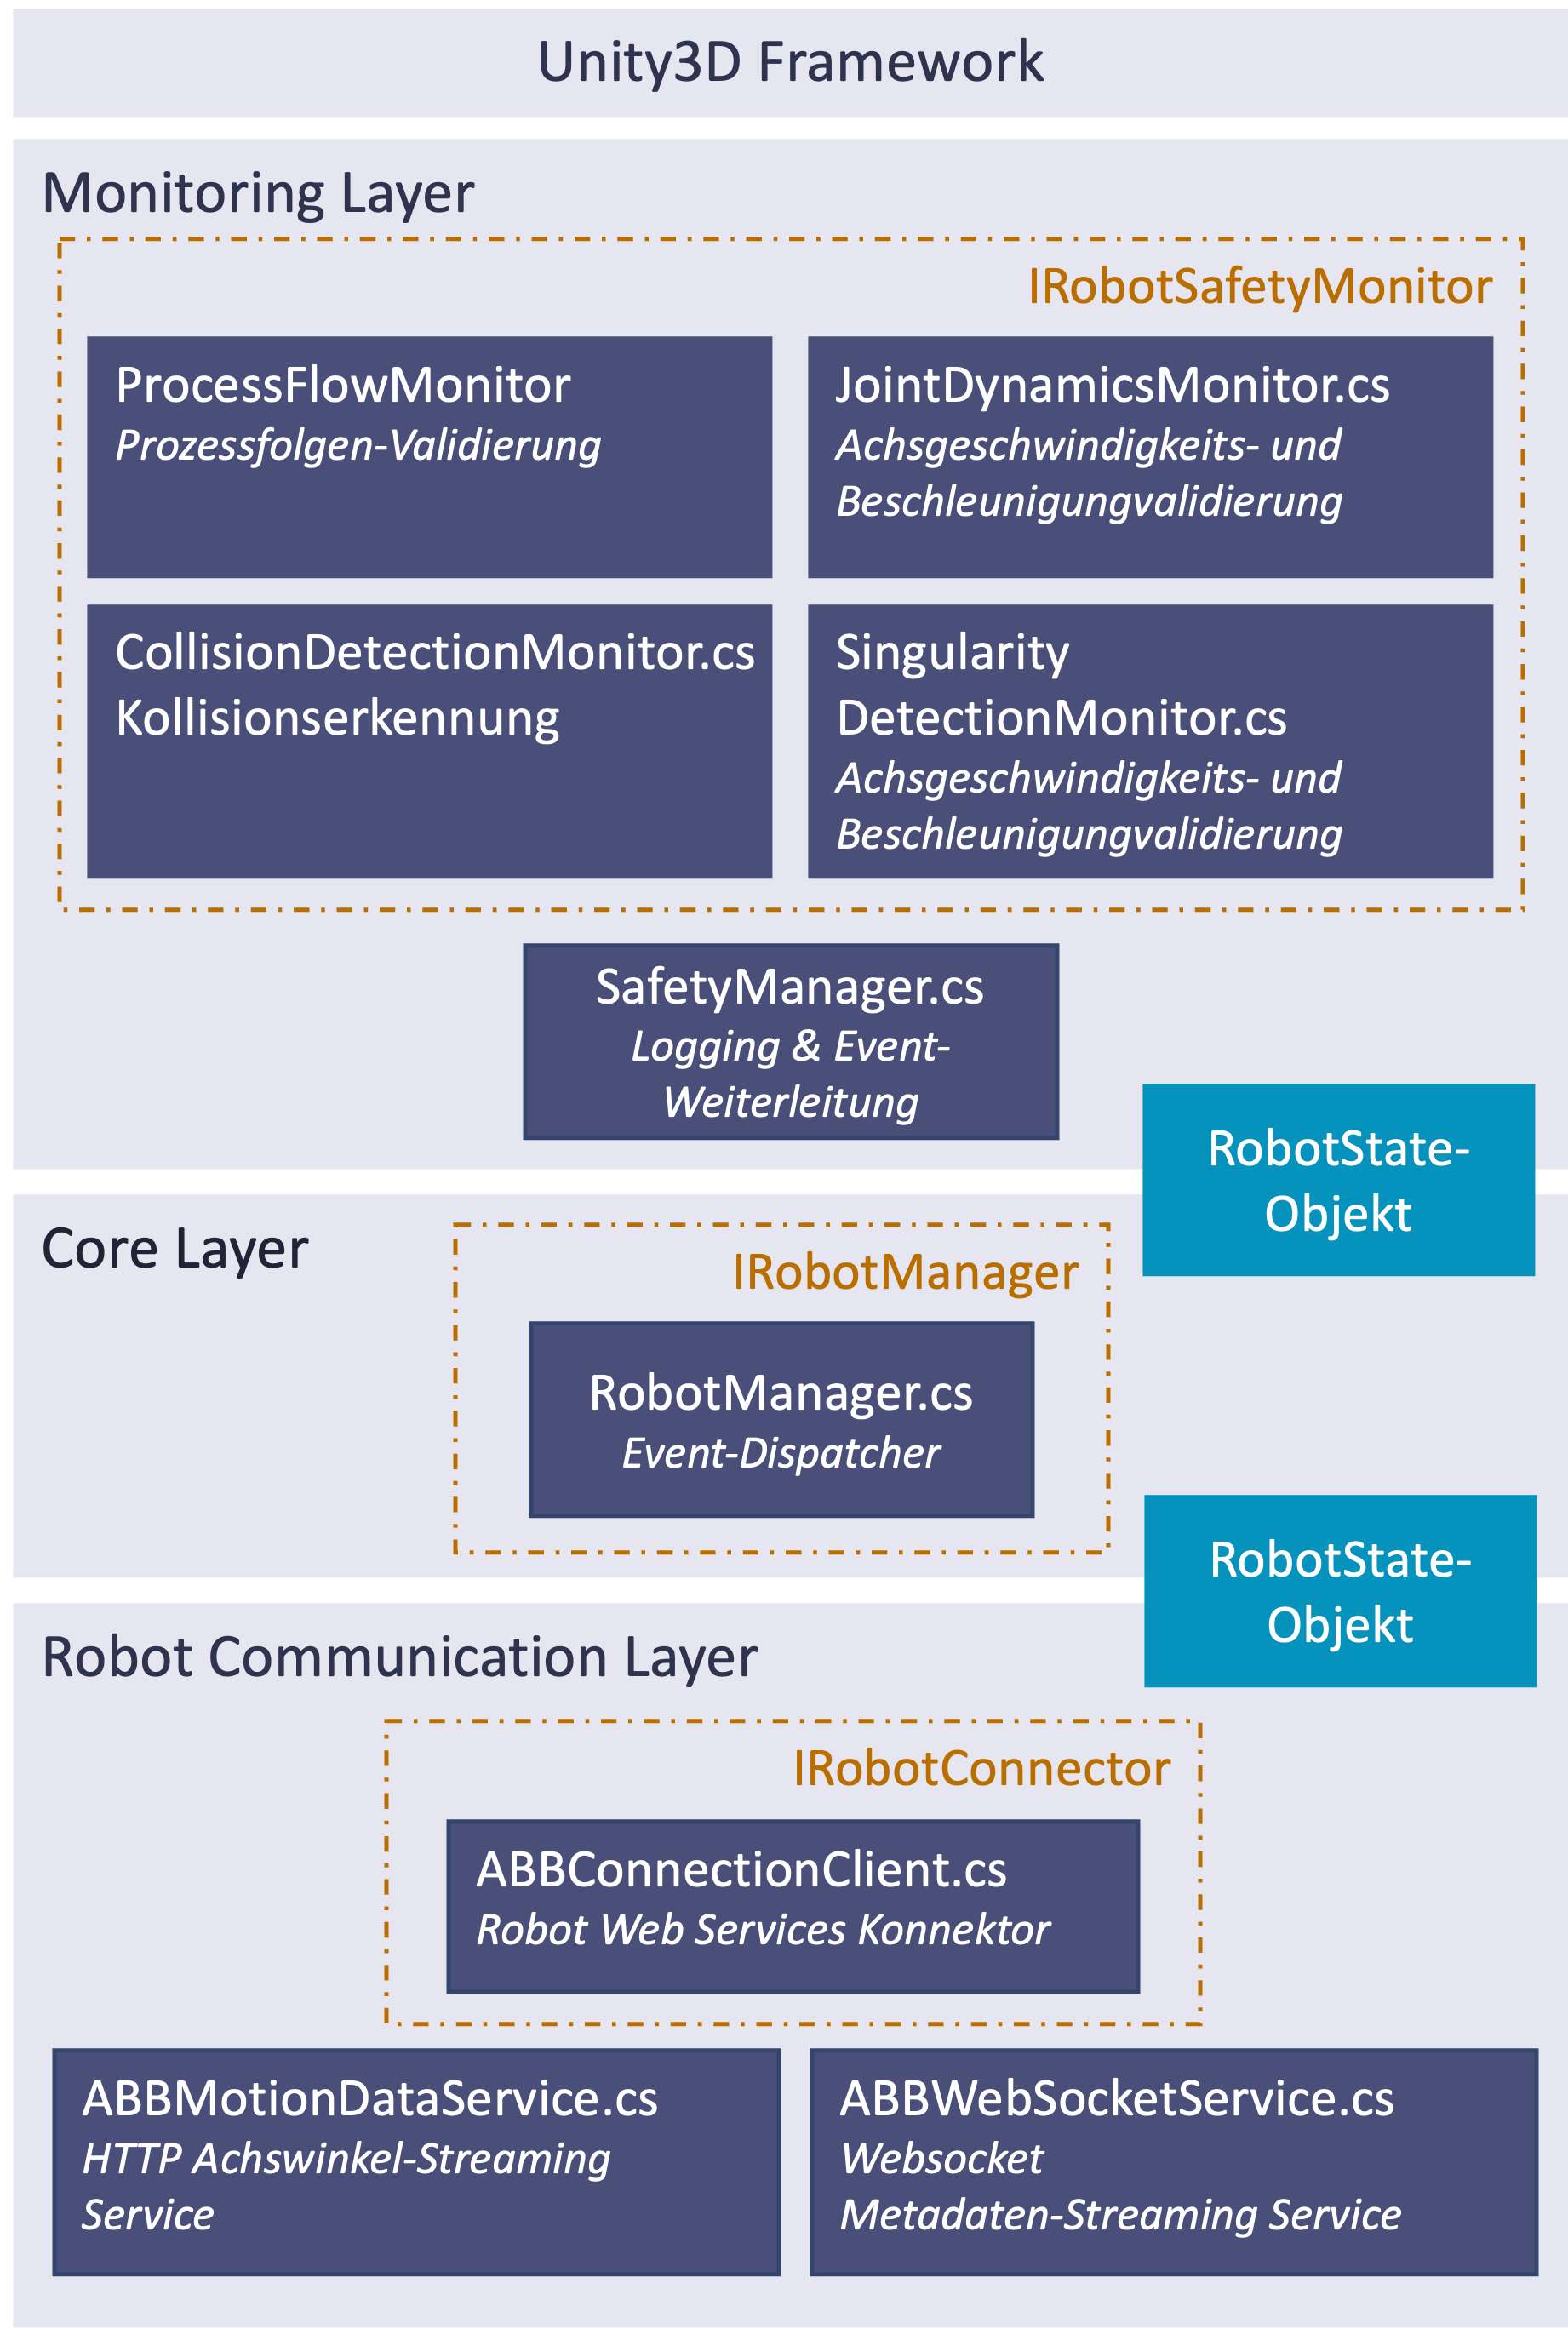
\includegraphics[width=10cm]{figures/LayerArchitekturFramework.png}
	\caption{Schichtenarchitektur des Frameworks. Orange umrandete Module implementieren formalisierte Interfaces (\texttt{IRobotSafetyMonitor}, \texttt{IRobotConnector}). Das \texttt{RobotState}-Objekt dient als gemeinsame Datenstruktur zwischen den Schichten.}
	\label{fig:layer_architecture}
\end{figure}

Die Architektur gliedert sich in vier logisch getrennte Schichten:

\begin{enumerate}
	\item \textbf{Unity3D Framework}: Bereitstellung der Simulationsumgebung und Physics-Engine
	\item \textbf{Monitoring Layer}: Implementierung der Sicherheitsmonitore
	\item \textbf{Core Layer}: Zentrales State-Management und Event-Koordination
	\item \textbf{Robot Communication Layer}: Adapter für herstellerspezifische Robotersteuerungen
\end{enumerate}

% Ergänzende Beschreibung der drei oberen Schichten. Die Layer werden
% jeweils kurz nach Zweck, Verantwortung und Schnittstellen eingeordnet,
% um eine einheitliche Detailtiefe herzustellen.

\paragraph{Unity3D Framework (Simulationsschicht)}
\begin{itemize}
	\item \textbf{Zweck}: Bereitstellung der Simulationslaufzeit.
	\item \textbf{Verantwortung}: Taktung des Systems (Update‑Loop), Szenenhosting und Bootstrap der Adapter. Abseits des Szenenlayouts und der Darstellung der Objekte soll hier keine tiefergehende Prozesslogik implementiert werden.
	\item \textbf{Schnittstellen}: Registrierung der Adapter über ein Dependency‑Injection‑Konzept; Monitore greifen nicht direkt auf Engine‑APIs, lediglich Collider-Objekte werden weitergegeben.
\end{itemize}

\paragraph{Core Layer}
\begin{itemize}
	\item \textbf{Zweck}: Domänenkern für den Roboterzustand und die Ereignisverteilung.
	\item \textbf{Verantwortung}: Aktualisierung des \texttt{RobotState}, Verteilung von Zustandsänderungen an registrierte Monitore (Observer) und Aggregation von \texttt{SafetyEvent}s.
	\item \textbf{Schnittstellen}: \texttt{RobotManager}, \texttt{RobotSafetyManager} und \texttt{RobotState} bilden die Kernklassen für Dispatch und Aggregation \vglcite[293\psq]{Gamma1994}.
\end{itemize}

\paragraph{Monitoring Layer}
\begin{itemize}
	\item \textbf{Zweck}: Kapselung der Prüfregeln als Policies für einzelne Fehlertypen (Kollision, Prozessfolge, Singularität, Dynamik).
	\item \textbf{Verantwortung}: Erzeugung normalisierter \texttt{SafetyEvent}s und Meldung von Grenzverletzungen.
	\item \textbf{Schnittstellen}: Einheitliches Kerninterface \texttt{IRobotSafetyMonitor} definiert die Bindung für alle Monitore.
\end{itemize}

Der \texttt{RobotManager} im Core Layer fungiert als zentraler
Event-Dispatcher, der Zustandsänderungen an alle registrierten
Monitoring-Komponenten propagiert. Diese Implementierung des Observer Patterns
ermöglicht eine lose Kopplung zwischen den
Komponenten\vglcite[293-303]{Gamma1994}: Die Sicherheitsmonitore müssen
lediglich das \texttt{IRobotSafetyMonitor}-Interface implementieren und können
zur Laufzeit dynamisch registriert oder entfernt werden, ohne andere Systemteile
zu beeinflussen.

Die in Abbildung \ref{fig:layer_architecture}
orange markierten Module definieren standardisierte Interfaces, die als Verträge
zwischen den Schichten dienen. Diese Interface-basierte Abstraktion realisiert
das Open-Closed-Prinzip, welches festlegt, dass Komponenten einerseits offfen
für Erweiterung sein sollen, andererseits geschlossen für
Veränderung\vglcite{Martin2003}: Neue Robotertypen können durch Implementierung
des \texttt{IRobotConnector}-Interfaces integriert werden, ohne den Core Layer
zu modifizieren. Analog können zusätzliche Sicherheitsmonitore über das
\texttt{IRobotSafetyMonitor}-Interface hinzugefügt werden. Diese
Architekturentscheidung gewährleistet, dass das System für Erweiterungen offen
bleibt, während die Kernfunktionalität stabil und unverändert bleibt.


Die Kommunikation zwischen den Schichten erfolgt ereignisgesteuert über das
\texttt{RobotState}-Objekt als gemeinsame Datenstruktur. Die Communication Layer
aktualisiert kontinuierlich den Roboterzustand durch WebSocket-Events für
Metadaten und HTTP-Polling für Bewegungsdaten. Der \texttt{RobotManager}
verteilt diese Zustandsänderungen asynchron an alle registrierten Observer.
Diese Event-Driven Architecture adressiert die Anforderungen an ein
erweiterbares und gleichzeitiges Nachrichtenfluss-Modell. So lassen sich Events
an mehrere Teilnehmer gleichzeitig weitergeben und verarbeiten, ohne dabei auf
den Processing-Zyklus zu warten. Weiterführend werden Events getrennt voneinader
verarbeitet, das heisst der Main-Thread muss nicht auf die Fertigstellung der
Abarbeitung von Events durch Empfänger warten.\vglcite[1\psqq]{hohpe2006}


Der \texttt{SafetyManager} aggregiert die von den Monitoren generierten
Sicherheitsereignisse und implementiert eine kontextabhängige Logging-Strategie.
Bei laufendem Roboterprogramm werden detaillierte JSON-Logs für spätere Analyse
erstellt, während im Idle-Zustand nur kritische Ereignisse in die Konsole
geloggt werden. Diese Differenzierung optimiert sowohl die Performance als auch
die Nachvollziehbarkeit von Sicherheitsvorfällen.


Die gewählte Schichtenarchitektur ermöglicht die unabhängige Entwicklung und
Testung einzelner Komponenten. Horizontale Erweiterungen (neue Monitore) und
vertikale Erweiterungen (neue Robotertypen) können ohne ungewollte Seiteneffekte auf
bestehende Komponenten implementiert werden.


\subsection{Robot Communcation Layer}
Die Robot Communication Layer organisiert die Kommunkation mit der zugrundeliegenden Robotersteuerung und
implentiert eine Interface des Typs IRobotConnector. Als Verbindungsclient
zwischen Unity und externer Schnittstelle des Robotersystems implementiert
dieser eine IRobotConnector Interface, welche als Vorlage für eine Anbindung an
eine Robotersteuerung jedes Typs fungiert und standartisierte Methoden
implementiert:

\begin{figure}[H]
	\inputminted[fontsize=\footnotesize]{csharp}{code-snippets/IRobotConnector.cs}
	\caption{Implementierung der IRobotConnector-Interface als Verbidung zwischen
		RobotState und Roboter-Controller}
\end{figure}

Eine Interface lässt sich anhand dieses Beispiels in \textbf{3
	Funktionsbereiche} aufteilen: Events, Attribute und Methoden.


Die Interface definiert \textbf{Events (Aktionen)} die bei definierten Zustandsänderungen
in der Laufzeit ausgeführt werden. Andere Bestandteile des Framework sind in der
Lage, ein Event zu abonnieren und eine Methode zu registrieren, welche ausgeführt
werden soll, wenn dieses Event auftritt. Ist dies der Fall, wird das
entsprechende Modul über die Änderung benachrichtigt und bekommt gegebenfalls
neue Daten zur Verfügung gestellt. Diese event-getriebene Kommunikation sorgt
dafür, dass einerseits alle Komponenten proaktiv auf den neusten Stand der Daten gebracht
und gehalten werden, andererseits aber keine ressourcenblockierenden Prozesse
ausgeführt werden müssen, um gegebenfalls Statusänderungen abzufragen.


Weiterführend definiert die Interface IRobotConnector \textbf{Attribute}, welche den
aktuellen Verbindungsstatus (verbunden = \texttt{true}, getrennt = \texttt{false}) speichern sowie das
State-Objekt des Roboters. Definiert durch die schreibgeschützten, automatisch
implementierte Eigenschaft mit einem Getter \textit{\{ get; \}} können Attribute
auch von ausserhalb des RobotConnectors abgefragt werden, jedoch nicht
überschrieben.


Zuletzt gibt die Interface die Methoden \textit{\textbf{Connect}} und \textit{\textbf{Disconnect}}
vor, welche hier die wichtigsten Methoden zum Verbinden und
Trennen von der jeweiligen Robotersteuerung darstellen.

Als initiale Komponente wird eine Verbindung zum
Controller eines Roboters benötigt, um den Roboter in Unity emulieren zu können
und Daten zu verarbeiten. Dazu wird hier mittels eines HTTP-Clients zur
Schnittstelle des RobotStudioSDKs über die API RobotWebServices (RWS) eine
Verbindung aufgebaut. Die Verbindung zu RobotWebServices ensteht durch einen
HTTP-Client und der Authentifizierung mit in RobotStudio festgelegten
Zugangsdaten. Anschliessend kann über einen erhaltenen Cookie die Verbindung
aufrecherhalten werden und aktuelle Daten über den Roboter sowohl abgefragt,
also auch der Roboter selbst gesteuert werden.\vglcite{robotwebservices2025}

Die RWS-Schnittstelle bietet einerseits die Möglichkeiten,
aktuellen Achswinkel und TCP-Werte (Tool Center Point) abzurufen, als auch
weitere Metadaten, wie das aktuell laufende Programm, den aktuellen Motorstatus
oder auch die Codezeile, welche aktuell vom Programmzeiger ausgeführt wird.
Weiterführend bietet RWS die Möglichkeit, aktuelle digitale und analoge
Signale abzurufen, was nötig ist, um den Greifer steuern zu können.

Bei den oben genannten Daten mit Ausnahme der Achswinkel handelt es sich um
Paramenter, welche sich im Laufe eines Programmablaufs vergleichsweise selten
verändern. Daher wird hier auf den Websockets-Endpunkt von RWS zugegriffen, um
innerhalb einer Duplex-Kommunikation sich verändernende Signale oder auch
Programmstati zu empfangen. Dazu wird mithilfe des HTTP-Clients eine Anfrage zur
Subscription auf verschiedene Parameter (bspw. den ProgrammPointer) gestellt,
und anschliessend eine Websockets-Session aufgebaut. Die Achswinkel werden
zeitgleich über eine asynchron endlosen Task in einer in Unity definierbaren
Frequenz abgefragt.

Der Client implementiert dabei die Interface IRobotConnector und gibt ein
RobotState-Objekt mit den empfangenen Daten an den RobotManager weiter, welcher hier
als zentraler Koordinator des aktuellen RobotState fungiert.


\paragraph{Event-Driven Architecture}
as System nutzt ein durchgängiges Event-System für lose Kopplung:
\begin{itemize}
	\item \texttt{OnRobotStateUpdated}: Zustandsänderungen
	\item \texttt{OnConnectionStateChanged}: Verbindungsstatus
	\item \texttt{OnSafetyEventDetected}: Sicherheitsereignisse
	\item \texttt{OnMotorStateChanged}: Motorstatusänderungen
\end{itemize}

\paragraph{SafetyEvent und RobotStateSnapshot}
Als für die Auswertung der Simulationsergebnisse relevantes Teil des Frameworks
wird die SafetyEvent-Klasse implementiert. Jedes Mal, wenn ein Ereignis,
welches mit der tatsächlichen Simluation eines Roboterprogramms zusammenhängt,
auftritt, wird ein SafetyEvent instanziert. Dieses wird initial von der
jeweiligen überwachenden Komponente (einem SafetyMonitor) instanziert und mit
dem aktuellsten RobotState als unveränderliches Objekt (RobotStateSnapshot) befüllt.
Weiterführend erhält es vom jeweiligen SafetyMonitor variierende
Kontextinformationen, die später für die Auswertung des Ereignisses verwendet
werden. Zusammenfassend bestehn ein SafetyEvent aus folgenden Komponenten:
\begin{itemize}
	\item \textbf{SafetyEvent}: Unveränderliches Value Object für Sicherheitsereignisse
	\item \textbf{RobotStateSnapshot}: Immutable Zustandserfassung zum Ereigniszeitpunkt
	\item \textbf{Ereignistypen}: Info, Warning, Critical mit konfigurierbaren Schwellwerten
	\item \textbf{Kontextdaten}: Vollständige Roboterzustandserfassung für Forensik
\end{itemize}

\paragraph{Einordnung}
Die folgenden Kapitel beschreiben die Implementierung der vier Monitore auf Basis
der zuvor skizzierten Schichten. In Kapitel~\ref{cap:Ergebnisse} werden die
Ergebnisse anhand gezielter Testszenarien dargestellt und in gekürzten
Log‑Auszügen (\texttt{minted}) veranschaulicht.
